\subsection{Overall}

Our testing showed that nearly all of the tested models yielded similar results, achieving approximately 80\% accuracy in our best predictions, with F-metric over 89\%.

The best results were achieved by more complex models (particularly neural networks, which were tested under numerous parameters.) Logistic Regression also yielded strong results, prompting us to consider other statistical methods for future testing.

We observed that a single perceptron neuron was significantly inferior to all of the other included models, yielding over 5\% deterioration in accuracy metrics. We believe this is caused by the rigid linear classification of perceptron, which other models compensate for.

\subsubsection{Random Forests}

As expected, ensemble learning from decision trees quickly over-fits training data. The overall generalization to test data was not impacted heavily, however it seems that it may be difficult to improve this model with further modifications to the input data.

        \begin{center}
        \begin{tabular}{| c | c || c | c | c | c |}
        \hline
        Dataset & Label & Accuracy & F1 & Precision & Recall \\
        \hline \hline
         Training & Default         & 100.0\% & 100.0\% & 100.0\% & 100.0\% \\
         Training & Paid in Full    &       & 100.0\% & 100.0\% & 100.0\% \\
         \hline
         Test & Default             & 80.5\% & 12.7\% & 53.8\% & 7.2\% \\
         Test & Paid in Full        &       & 89.0\% & 81.2\% & 98.5\% \\
         \hline
        \end{tabular}
        \end{center}

\subsubsection{SVM}

The SVM model predicted as well as other models despite its linear nature, though did not quite match more expressive non-linear models.

        \begin{center}
        \begin{tabular}{| c | c || c | c | c | c |}
        \hline
        Dataset & Label & Accuracy & F1 & Precision & Recall \\
        \hline \hline
         Training & Default         & 80.1\% & 3.3\% & 50.5\% & 1.7\% \\
         Training & Paid in Full    &       & 88.9\% & 80.3\% & 99.6\% \\
         \hline
         Test & Default             & 80.3\% & 3.4\% & 48.7\% & 1.8\% \\
         Test & Paid in Full        &       & 89.0\% & 80.5\% & 99.5\% \\
         \hline
        \end{tabular}
        \end{center}

\subsubsection{Logistic Regression}

This model yielded the best overall results (though nearly identical to our final keras neural network implementation.)

        \begin{center}
        \begin{tabular}{| c | c || c | c | c | c |}
        \hline
        Dataset & Label & Accuracy & F1 & Precision & Recall \\
        \hline \hline
         Training & Default         & 80.3\% & 9.1\% & 55.3\% & 5.0\% \\
         Training & Paid in Full    &       & 88.9\% & 80.7\% & 99.0\% \\
         \hline
         Test & Default             & 80.5\% & 9.4\% & 55.1\% & 51.2\% \\
         Test & Paid in Full        &       & 89.1\% & 81.0\% & 99.0\% \\
         \hline
        \end{tabular}
        \end{center}

\subsection{Perceptron}

The single perceptron node was the worst predictor of the tested methods. It seems that this model may be too rigidly linear for the data.

        \begin{center}
        \begin{tabular}{| c | c || c | c | c | c |}
        \hline
        Dataset & Label & Accuracy & F1 & Precision & Recall \\
        \hline \hline
         Training & Default         & 74.2\% & 19.4\% & 25.6\% & 15.5\% \\
         Training & Paid in Full    &       & 84.6\% & 80.9\% & 88.8\% \\
         \hline
         Test & Default             & 74.4\% & 19.8\% & 26.0\% & 16.0\% \\
         Test & Paid in Full        &       & 84.8\% & 81.2\% & 88.8\% \\
         \hline
        \end{tabular}
        \end{center}

\subsubsection{Neural Net}

Of the numerous settings modeled in keras, we found that increasing the complexity of the model did not yield much improvement in our results. As such, we favored a somewhat simpler model of only $3 \times 20$ hidden features.

The following results were generated by the referenced model of 3 hidden layers, 20 nodes per layer:

        \begin{center}
        \begin{tabular}{| c | c || c | c | c | c |}
        \hline
        Dataset & Label & Accuracy & F1 & Precision & Recall \\
        \hline \hline
         Test & Paid in Full        & 80.4 & 89.0\% & 81.0\% & 98.7\% \\
         \hline
        \end{tabular}
        \end{center}

This figure demonstrates the change in outcome as we increased complexity of the network. It appears that overfitting begins to occur after a width of only 30 neurons with training error continuing to decrease but the generalization performance fluctuating.

\begin{figure}[h!]
	\centering
	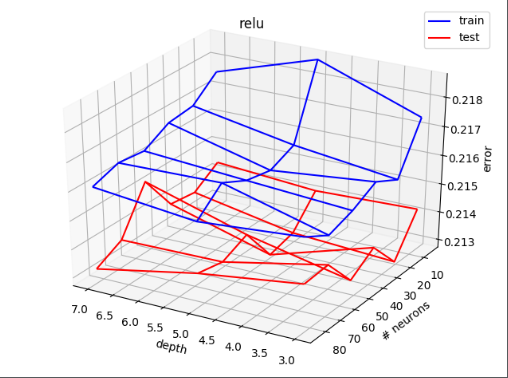
\includegraphics[width=10cm, height=7cm]{neural_nets.png}
	\caption{Train and Test Error for Various Architectures}
	\label{fig:neural_net}
\end{figure}
